\documentclass[12pt,twoside]{report}

% some definitions for the title page
\newcommand{\reporttitle}{A C Memory Model for use with Concolic Testing}
\newcommand{\reportauthor}{Charles Loveman}
\newcommand{\supervisor}{Daniel Schemmel}
\newcommand{\reporttype}{Type of Report/Thesis}
\newcommand{\degreetype}{Type of degree} 

% load some definitions and default packages
%%%%%%%%%%%%%%%%%%%%%%%%%%%%%%%%%%%%%%%%%
% University Assignment Title Page 
% LaTeX Template
% Version 1.0 (27/12/12)
%
% This template has been downloaded from:
% http://www.LaTeXTemplates.com
%
% Original author:
% WikiBooks (http://en.wikibooks.org/wiki/LaTeX/Title_Creation)
%
% License:
% CC BY-NC-SA 3.0 (http://creativecommons.org/licenses/by-nc-sa/3.0/)
% 
%
%%%%%%%%%%%%%%%%%%%%%%%%%%%%%%%%%%%%%%%%%
%----------------------------------------------------------------------------------------
%	PACKAGES AND OTHER DOCUMENT CONFIGURATIONS
%----------------------------------------------------------------------------------------
\usepackage[a4paper,hmargin=2.8cm,vmargin=2.0cm,includeheadfoot]{geometry}
\usepackage{textpos}
\usepackage{natbib} % for bibliography
\usepackage{tabularx,longtable,multirow,subfigure,caption}%hangcaption
\usepackage{fncylab} %formatting of labels
\usepackage{fancyhdr} % page layout
\usepackage{url} % URLs
\usepackage[english]{babel}
\usepackage{amsmath}
\usepackage{graphicx}
\usepackage{dsfont}
\usepackage{epstopdf} % automatically replace .eps with .pdf in graphics
\usepackage{backref} % needed for citations
\usepackage{array}
\usepackage{latexsym}
\usepackage[pdftex,pagebackref,hypertexnames=false,colorlinks]{hyperref} % provide links in pdf

\hypersetup{pdftitle={},
  pdfsubject={}, 
  pdfauthor={},
  pdfkeywords={}, 
  pdfstartview=FitH,
  pdfpagemode={UseOutlines},% None, FullScreen, UseOutlines
  bookmarksnumbered=true, bookmarksopen=true, colorlinks,
    citecolor=black,%
    filecolor=black,%
    linkcolor=black,%
    urlcolor=black}

\usepackage[all]{hypcap}


%\usepackage{color}
%\usepackage[tight,ugly]{units}
%\usepackage{float}
%\usepackage{tcolorbox}
%\usepackage[colorinlistoftodos]{todonotes}
% \usepackage{ntheorem}
% \theoremstyle{break}
% \newtheorem{lemma}{Lemma}
% \newtheorem{theorem}{Theorem}
% \newtheorem{remark}{Remark}
% \newtheorem{definition}{Definition}
% \newtheorem{proof}{Proof}


%%% Default fonts
\renewcommand*{\rmdefault}{bch}
\renewcommand*{\ttdefault}{cmtt}



%%% Default settings (page layout)
\setlength{\parindent}{0em}  % indentation of paragraph

\setlength{\parindent}{0em}  % indentation of paragraph

\setlength{\headheight}{14.5pt}
\pagestyle{fancy}
\renewcommand{\chaptermark}[1]{\markboth{\chaptername\ \thechapter.\ #1}{}} 
%\fancyhead[RO]{\sffamily \textbf{\thepage}} %Page no.in the right on even pages
%\fancyhead[LE]{\sffamily \textbf{\thepage}} %Page no. in the left on odd pages

\fancyfoot[ER,OL]{\thepage}%Page no. in the left on
                                %odd pages and on right on even pages
\fancyfoot[OC,EC]{\sffamily }
\renewcommand{\headrulewidth}{0.1pt}
\renewcommand{\footrulewidth}{0.1pt}
\captionsetup{margin=10pt,font=small,labelfont=bf}


%--- chapter heading

\def\@makechapterhead#1{%
  \vspace*{10\p@}%
  {\parindent \z@ \raggedright \sffamily
    \interlinepenalty\@M
    \Huge\bfseries \thechapter \space\space #1\par\nobreak
    \vskip 30\p@
  }}

%--- chapter heading

\def\@makechapterhead#1{%
  \vspace*{10\p@}%
  {\parindent \z@ \raggedright \sffamily
        %{\Large \MakeUppercase{\@chapapp} \space \thechapter}
        %\\
        %\hrulefill
        %\par\nobreak
        %\vskip 10\p@
    \interlinepenalty\@M
    \Huge\bfseries \thechapter \space\space #1\par\nobreak
    \vskip 30\p@
  }}

%---chapter heading for \chapter*  
\def\@makeschapterhead#1{%
  \vspace*{10\p@}%
  {\parindent \z@ \raggedright
    \sffamily
    \interlinepenalty\@M
    \Huge \bfseries  #1\par\nobreak
    \vskip 30\p@
  }}	
\allowdisplaybreaks

% load some macros
% Here, you can define your own macros. Some examples are given below.

\newcommand{\R}[0]{\mathds{R}} % real numbers
\newcommand{\Z}[0]{\mathds{Z}} % integers
\newcommand{\N}[0]{\mathds{N}} % natural numbers
\newcommand{\C}[0]{\mathds{C}} % complex numbers
\renewcommand{\vec}[1]{{\boldsymbol{{#1}}}} % vector
\newcommand{\mat}[1]{{\boldsymbol{{#1}}}} % matrix


\usetikzlibrary{shapes}
%\usepackage[
%backend=biber,
%style=apa,
%sorting=ynt
%]{biblatex}
%\addbibresource{references.bib}
\bibliographystyle{abbrv}
% load title page
\begin{document}
% Last modification: 2015-08-17 (Marc Deisenroth)
\begin{titlepage}

\newcommand{\HRule}{\rule{\linewidth}{0.5mm}} % Defines a new command for the horizontal lines, change thickness here

%----------------------------------------------------------------------------------------
%	LOGO SECTION
%----------------------------------------------------------------------------------------


\includegraphics[width = 4cm]{./figures/imperial}\\[0.5cm] 

\center % Center everything on the page
 
%----------------------------------------------------------------------------------------
%	HEADING SECTIONS
%----------------------------------------------------------------------------------------

\textsc{\LARGE \reporttype}\\[1.5cm] 
\textsc{\Large Department of Computing}\\[0.5cm] 
\textsc{\large Imperial College of Science, Technology and Medicine}\\[0.5cm] 

%----------------------------------------------------------------------------------------
%	TITLE SECTION
%----------------------------------------------------------------------------------------

\HRule \\[0.4cm]
{ \huge \bfseries \reporttitle}\\ % Title of your document
\HRule \\[1.5cm]
 
%----------------------------------------------------------------------------------------
%	AUTHOR SECTION
%----------------------------------------------------------------------------------------

\begin{minipage}{0.4\textwidth}
\begin{flushleft} \large
\emph{Author:}\\
\reportauthor % Your name
\end{flushleft}
\end{minipage}
~
\begin{minipage}{0.4\textwidth}
\begin{flushright} \large
\emph{Supervisor:} \\
\supervisor % Supervisor's Name
\end{flushright}
\end{minipage}\\[4cm]




%----------------------------------------------------------------------------------------


%----------------------------------------------------------------------------------------
%	DATE SECTION
%----------------------------------------------------------------------------------------

{\large \today} % Date, change the \today to a set date if you want to be precise


\vfill % Fill the rest of the page with whitespace
Submitted in partial fulfillment of the requirements for the \degreetype~of Imperial College London

\end{titlepage}



% page numbering etc.
\pagenumbering{roman}
\clearpage{\pagestyle{empty}\cleardoublepage}
\setcounter{page}{1}
\pagestyle{fancy}

%%%%%%%%%%%%%%%%%%%%%%%%%%%%%%%%%%%%
%\begin{abstract}
%Your abstract.
%\end{abstract}

%\cleardoublepage
%%%%%%%%%%%%%%%%%%%%%%%%%%%%%%%%%%%%
%\section*{Acknowledgments}
%Comment this out if not needed.

%\clearpage{\pagestyle{empty}\cleardoublepage}

%%%%%%%%%%%%%%%%%%%%%%%%%%%%%%%%%%%%
%--- table of contents
\fancyhead[RE,LO]{\sffamily {Table of Contents}}
\tableofcontents 


%\clearpage{\pagestyle{empty}\cleardoublepage}
\pagenumbering{arabic}
\setcounter{page}{1}
\fancyhead[LE,RO]{\slshape \rightmark}
\fancyhead[LO,RE]{\slshape \leftmark}

%%%%%%%%%%%%%%%%%%%%%%%%%%%%%%%%%%%%
\chapter{Introduction}
%1-3 pages
% It’s a good idea to try to write the introduction to your final report early on in the project. However, you will find it hard, as you won’t yet have a complete story and you won’t know what your main contributions are going to be. However, the exercise is useful as it will tell you what you don’t yet know and thus what questions your project should aim to answer. For the interim report this section should be a short, succinct, summary of the project’s main objectives. Some of this material may be re-usable in your final report, but the chances are that your final introduction will be quite different.  You are therefore advised to keep this part of the interim report short, focusing on the following questions: What is the problem, why is it interesting and what’s your main idea for solving it?  (DON'T use those three questions as subheadings however!  The answers should emerge from what you write.)

Program vulnerabilities can be hugely damaging and the annual cost of software exploits increases year on year. There is a wide range of possible exploits, but one of the most commonly exploited classes of vulnerabilities are caused by memory bugs. These bugs occur when the program violates the rules that govern how a program may interact with memory, called the memory model of the programming language, and these bugs can be very difficult to find. 

Each programming language uses a different memory model, but there is a general model used by many programming languages that is particularly vulnerable. If we consider the memory address space to be a set of bytes, each memory object can be described by a location and a set of bytes that makes up the memory object which is a subset of the address space. Valid memory accesses must be fully contained within a single memory object.

By imposing the minimum requirements on how the program validates its own behaviour, violations of this model can be hidden or cause unexpected behaviour. Despite these issues, this family of programming languages includes C and C++, two of the most popular languages in the world. They take advantage of the simple rules to produce highly efficient programs and have been used to implement almost all high performance software including operating systems and other critical systems.

Due to the inherently dynamic nature of memory operations in this memory model, we cannot verify statically if a program violates the memory model. Instead, we need to implement a dynamic system to check if the model has been violated at runtime. This is similar to the behaviour of memory sanitizers like ASAN, which instrument the target program so that when it is run the memory errors are reported. 

Despite the existence of tools like ASAN which can detect memory errors, manual and randomised testing campaigns can still miss bugs in programs. The reason is that if you don't guess an input which triggers the bug, it cannot be reported. Concolic execution tackles this problem by recording the constraints that had to be met on the input to the program to take a particular path through the program and uses an SMT solver to find new inputs which take different paths through the program. This gives us an automated method to increase test coverage and generate new inputs which could detect bugs.

For concolic execution to construct these constraints, we need to store metadata regarding the operations that have been performed on the values of the program during execution. As we already store metadata about program values, this can be extended to add support for a memory model checker which will validate each memory access the target program performs. We design and implement a memory model checker into a prototype concolic execution framework called CCF.

\begingroup
\let\clearpage\relax
\chapter{Ethical Issues}
\endgroup
 %Ethical issues (where necessary - 1-2 pages). Are there wider ethical, legal, professional and societal issues surrounding your project and the accompanying research? If there are, please discuss these. You should use the ethics checklist as the basis for this discussion.
 %Just go through the checklist, no big problems here.

 As a computing project, this project utilises computers which can have a negative impact on the environment. However, we expect that the benefit gained by detecting program errors will outweigh the environmental impact of running the software. The software produced will make use of open source software, which will not infringe on their copyright.

 As concolic execution software can find bugs in programs, a malicious attacker who obtained access to a victims source code could use the software to find vulnerabilities in the victim's software which would allow them to cause harm. However, as the program is publicly available to the victim also, they should be able to find and fix this vulnerability with the help of the program and it is worth noting that the software will not create any new vulnerabilities, only expose ones that already exist.


%%%%%%%%%%%%%%%%%%%%%%%%%%%%%%%%%%%%
\chapter{Background}
%10-20 pages
%The background section of the report should set the project into context by relating it to existing published work which you read at the start of the project when your approach and methods were being considered. There are usually many ways of solving a given problem, and you shouldn't just pick one at random. Describe and evaluate as many alternative approaches as possible. The published work may be in the form of research papers found in the academic literature, articles, text books, technical manuals, or even existing software or hardware of which you have had hands-on experience. Your must acknowledge the sources of your inspiration. You are expected to have seen and thought about other people's ideas; your contribution will be putting them into practice in some other context. However, avoid plagiarism: if you take another person's work as your own and do not cite your sources of information/inspiration you are being dishonest. When referring to other pieces of work, cite the sources where they are referred to or used, rather than just listing them at the end. Accidental plagiarism or not knowing how to cite and reference is not a valid reason for plagiarism. Make sure you read and digest the Department's plagiarism document .

%In writing the Background chapter you must demonstrate your ability to analyse, synthesise and apply critical judgement. Analysis is shown by explaining how the proposed solution operates in your own words as well as its benefits and consequences. Synthesis is shown through the organisation of your Related Work section and through identifying and generalising common aspects across different solutions. Critical judgement is shown by discussing the limitations of the solutions proposed both in terms of their disadvantages and limits of applicability.

Every programming language has a specification for how a program may interact with memory, although for some languages this is not always clearly defined. This definition of a set of rules regarding memory interactions is called a memory model and a violation of these rules is a memory bug. As a memory bug occurs due to a violation of the rules of the programming language, memory bugs are undeniably incorrect. This makes memory bugs a viable target for automated testing as we know that if we find a memory bug it is a real bug in the program.

The memory model of many programming languages can be modelled with a general memory model. We define the address space of a program to be the set of bytes that can be accessed by the program. Although these languages may have many different types of objects, we define the representation of the object in memory as a memory object. A memory object only has a location and set of bytes, which must be a subset of the address space. It is important to note that memory objects have no internal structure and cannot be defined recursively. On most architectures, the set of bytes allocated to a memory object will be contiguous, although we do not require this for the memory model.

Bytes in memory can either be allocated, which means they are an element of exactly one live memory object, or they are unallocated, which means they are not contained in any memory object. A valid allocation takes a set of unallocated bytes, and constructs a new memory object that contains only those bytes. A valid deallocation takes a set of bytes which is equal to the set of bytes allocated to a single memory object and removes the memory object, leaving the set of bytes unallocated. A valid memory access takes a set of allocated bytes, which are all contained within the same memory object.

\section{Checking a Memory Model}
The AddressSanitizer \cite{180957} (ASAN) is a dynamic memory model checker, which means that memory bugs can only be reported when the program is executed. As ASAN needs to modify the internal behaviour of the system under test (SUT), it instruments the SUT at compile time to insert behaviour whenever the SUT accesses memory. This allows it to monitor all memory interactions of the program and check if the memory model is violated.

The memory model used by ASAN is similar to the one described above. This model does not store memory object metadata inside of the memory objects themselves. In fact, given only a set of bytes there is no way to determine if the bytes are allocated or unallocated, or what memory object they are allocated to. As a result, ASAN stores additional metadata about every allocated byte so that it can verify if the memory model has been violated.

To check a memory model we need to monitor the memory allocations, deallocations, and memory accesses. When memory is allocated we need verify that all the bytes to be allocated are currently unallocated. As the memory model does not allow the user to request the addresses at which bytes are allocated this issue is generally avoided. On an allocation, ASAN will update its metadata to mark the bytes as allocated.

When memory is deallocated we need to check that all the bytes belong to the same object. ASAN accomplishes this by checking its metadata to see if all the bytes are allocated and ensuring that the memory objects are spaced apart with redzones to check if the deallocation spans between memory objects.

When memory is accessed we need to check that all the bytes belong to the same object. ASAN accomplishes this in the same way as with deallocations. All we need to check the memory model is to store metadata for each object and then check any memory accesses against the stored metadata.

\section{Finding New Inputs}
Although ASAN is a powerful tool for reporting memory model violations, it only works if the program input provided triggers a memory bug to occur. The number of possible inputs grows exponentially with the size of the input data, so the difficulty of finding inputs that trigger bugs also grows exponentially.

A single program execution can be described by which direction is taken at each branch encountered. This is called a path in the program. When testing we would like to cover all paths in the program, however, the number of paths grows exponentially with the number of branches. This means covering every path is often infeasible.

The majority of program testing is done using manually written tests \cite{8400261}. We can write test programs which execute part or all of the SUT with set input parameters, to examine the behaviour of the program and ensure that the execution performs as expected. Testing has many advantages, it is easy to set up and all modern programming languages will have extensive support for writing test cases. Furthermore, tests can be written as the program grows and develops to create a suite of tests that describes the intended behaviour of the program. However, testing has a key problem, where as the program grows the number of possible execution paths through program can grow exponentially. As a single test only follows one path through the program, you would need to manually write an exponential number of test cases to cover the full behaviour of the program. As a result, test suites for real software will not cover every possible path, potentially allowing bugs to remain in the program.

Randomised testing was developed to build upon manual testing by automatically generating test cases. Also called Fuzzing \cite{10.1145/96267.96279}, testing programs with random inputs has been able to find many bugs in long running software projects like GCC \cite{csmith, aflwhitepaper}. The effectiveness of random testing comes from the ability to search a greater number of paths compared to manual testing and a random test can avoid the biases that the test author may hold and search the whole input space fairly. However, in a large program some paths will only be reached from a small section of the input space and randomised testing finds paths in proportion to how many inputs take the path. This means that random testing is unlikely to find bugs on low probability paths.

An alternative to random testing is concolic execution, which uses a guided search to find new inputs.
Concolic execution has a higher overhead compared to random testing so the proportion of the input space searched will be lower but this trade off is made in favour of finding inputs that should take new program paths. This means that concolic execution should explore a new path with every input tried, although implementation details means this may not always occur in practice.

\section{Concolic Execution}
\begin{figure}
    \centering
    \begin{minipage}{0.3\textwidth}
    %if(x < 0) {x = 0;}; if (x > 5) {abort;}
\begin{lstlisting}[language=C]
int clamp(int* arr, int i) {
    if (arr[i] < 0) {
        return 0;
    }
    if (arr[i] > 5) {
        abort();
    }
    if (arr[i] > 10) {
        return 10;
    }
    return arr[i];
}
\end{lstlisting}
    \end{minipage}
    \caption{This program accesses element $i$ of array $arr$ and clamps the value between 0 and 10. However, if the value is greater than 5 then the program will crash.}
    \label{clamp}
\end{figure}

\tikzstyle{process} = [rectangle, minimum width=1cm, minimum height=0.5cm, text centered, draw=black, fill=orange!30]
\tikzstyle{arrow} = [thick,->]
\begin{figure}
    \centering
    \begin{minipage}{0.9\textwidth}
    %don't do x = value, just do x = lambda everywhere
    \begin{tikzpicture}[node distance=1.5cm]
        \node (root) [process] {$arr[i] < 0$};
        \node (node1) [process, below of=root, xshift=1.8cm] {SAT};
        \node (node2) [process, below of=root, xshift=-1.8cm] {$arr[i] > 5$};
        \node (node3) [process, below of=node2, xshift=-1.8cm] {$arr[i] > 10$};
        \node (node4) [process, below of=node3, xshift=1.8cm] {UNSAT};
        \node (node5) [process, below of=node3, xshift=-1.8cm] {SAT};
        \draw [arrow] (root) -- node[right=10pt] {$\{\lambda < 0\}$} (node1);
        \draw [arrow] (root) -- node[left=10pt] {$\{\neg(\lambda < 0)\}$} (node2);
        \draw [arrow] (node2) -- node[left=10pt] {$\{\neg(\lambda < 0), \neg(\lambda > 5)\}$} (node3);
        \draw [arrow] (node3) -- node[right=10pt] {$\{\neg(\lambda < 0), \neg(\lambda > 5), \lambda > 10\}$} (node4);
        \draw [arrow] (node3) -- node[left=10pt] {$\{\neg(\lambda < 0), \neg(\lambda > 5),\neg(\lambda > 10)\}$} (node5);
    \end{tikzpicture}
    \end{minipage}
    \caption{Execution paths in clamp function after 2 executions, with $arr[i] = \lambda$}
    \label{fig:clamp2}
\end{figure}

Suppose that you are interested in testing to see if the program in Figure \ref{clamp} can crash and through random testing you have tried the input $arr = (-5), \, i = 0$ and found that the program did not crash and returned 0. If you were only doing random testing then the next step would be to pick completely random values of $arr$ and $i$ and hope that you could get a different result. Concolic execution gives us a method to take the results of previous executions to select more interesting inputs to try.

We assign a symbolic expression to represent the value of the inputs of the program. For example, let $arr[i] = \lambda$, where $\lambda$ could take any integer value. Then we run the program with a concrete input, such as $arr[i] = -5$. Whenever a variable is assigned we additionally compute a symbolic expression to represent its new value and when the execution branches we record the conditions required to take the branch as a constraint on the symbolic values.

When we reach the branch $arr[i] < 0$, we can evaluate the condition concretely to determine if the branch will be taken. As $-5 < 0$ is true, the branch will be taken. Additionally, we record the constraint $\lambda < 0$. This means that in order to take this path through the program, the input must satisfy the expression $\lambda < 0$. We call the sequence of constraints recorded for a single path the path constraint.

We can generate an input which takes a new path by taking the path constraint and negating the final constraint. Here we only have one constraint so the new path constraint is $\{\neg(\lambda < 0)\}$. We can use a Satisfiability Modulo Theories (SMT) solver to find an input satisfying the constraint. It could return any number greater than or equal to 0, lets take 3 for this example.

After executing the program with the input $arr[i] = 3$, we get the path constraint $\{\neg(\lambda < 0), \neg(\lambda > 5), \neg(\lambda > 10)\}$. Negating the final constraint gives us $\{\neg(\lambda < 0), \neg(\lambda > 5), \lambda > 10\}$, but when we query the SMT solver it will give us the result UNSAT. This means there is no input which takes that path through the program. Figure \ref{fig:clamp2} shows the paths explored in an execution tree. To find the next input you would walk up the tree and query the SMT solver for $\{\neg(\lambda < 0), \lambda > 5\}$. Executing the new input should find the crash in the program.

This process is called concolic execution and is a type of symbolic execution. Concolic is a portmanteau of Concrete and Symbolic, referring to how in concolic execution variables have concrete values and symbolic expressions. We have seen how concolic execution can be used to efficiently construct and explore the execution tree of a program. 

Symbolic execution was developed in the 1970s \cite{10.1145/800027.808444, 10.1145/360248.360252, 1702443, 10.1145/800027.808445} as a way to test programs. 'Symbolic' means that the inputs given to the SUT do not have a single concrete value but instead each input can take a set of possible values. For example, let $x = \lambda$, where $\lambda$ is a symbolic value with possible values $1,2,3$. Then after executing $x = x + 1$, $x$ will equal the symbolic expression $\lambda + 1$ with the possible values $2,3,4$. In this way all the operations of a programming language can be extended to act on symbolic values.

\subsection{Determining Branch Conditions}
In order to determine if a branch can be taken, a Satisfiability Modulo Theory (SMT) solver \cite{Barrett2018} is used. These solvers extend Satisfiability (SAT) solvers to allow the use of background theories for greater expressibility. A SAT solver \cite{10.1007/978-3-540-24605-3_37} takes a logical formula and determines if there is an assignment to the boolean variables in the formula that will result in the formula being true. 
 
%is it natural`??
%quantifier free bitvectors and arrays, fp?
%need to talk about memory in symbolic execution

To describe program behaviour using only boolean variables is quite difficult, but using an SMT solver allows us to use the Quantifier-Free Bitvector theory, which lets us describe program behaviour using operations on fixed size bitvectors. This is more natural as program constructs like integers are typically represented in a computer as a bitvector, so operating with bitvectors allows us to put conditions on data operations more directly. We have to use the Quantifier-Free theory as introducing quantifiers makes the theory undecidable.

%An important theory for modelling the use of memory is the array theory \cite{10.1007/978-3-642-00768-2_16} which can be used to model changes to an array of values. This can greatly reduce the number of boolean variables required as representing each memory cell with its own variable would produce a huge number of variables which would slow down the solver greatly. We're interested in producing solutions as quickly as possible to explore more paths through the program, so the SMT solver used is important to get good results.

\subsection{Concolic Execution}
Concolic Execution is a program testing technique that combines symbolic execution with concrete execution \cite{217563}.
Concolic execution can be considered an offline version of symbolic execution. We select an input and follow a single path through the program. At each branch we encounter, we record the conditions on the symbolic input required for the branch. Once the execution terminates, we select one branch condition and reverse it, giving a new program path. Then we use an SMT solver to find an input that satisfies the branch conditions to get an input that will take the new path. By executing this loop repeatedly, we can search the tree of paths efficiently.

A concolic executor exploring Figure \ref{fig:foopaths} would select a random input initially, for example 6. In execution it would reach both the $x < 0$ and $x > 5$ branch nodes, finally reaching the $x = 5$ output. Then it would randomly select a condition, for example $x > 5$, and determine if there is an input that would take the same path up to this point, but then take the other direction. This gives the condition $\neg(x < 0) \wedge \neg(x > 5)$, which an SMT solver can solve to produce a satisfying assignment of $3$. The solver would then run a new execution with the input $x = 3$.

Concolic execution should reach a higher test throughput than symbolic execution, as the system under test is executed natively. This means each input executes faster and we should be able to explore a greater portion of the execution tree. At each symbolic branch symbolic execution has to fork its process to explore each side of the branch, this creates a higher overhead compared to concolic execution.

In symbolic execution the SMT solver is queried at each symbolic branch to determine if there are satisfying inputs that will take each side of the branch. In concolic execution the condition expression takes a concrete value and can branch immediately. Instead of querying the solver at each branch, the solver is queried once with all branch condition for a path to determine if an input exists. This should reduce the number of SMT queries made which will improve performance.

In symbolic execution constraints on the symbolic state of the program are produced automatically each time a symbolic branch is taken. This helps to avoid doing redundant work by exploring an unsatisfiable path. In concolic execution we use concrete values for execution, so we need to perform additional work to determine the constraints required to take the current execution path. To do this we need to record the symbolic expressions produced for each value calculated from a symbolic value and from this we can produce symbolic expressions constraining the inputs.

As concolic execution only tests with concrete inputs, we get a guarantee that any memory bugs found are real and can be reproduced from the same input (assuming no non-determinism). This can simplify the design of the memory model implementation, as the implementation only needs to detect if a memory access has concretely violated the memory model. This is different in symbolic execution where the memory model implementation needs to answer the question of could the memory access have been invalid. However, the memory model must be able to produce constraints on the access which amounts to mostly the same thing, so this may not be a large advantage.

\subsection{CCF}
% prototype
% missing some features e.g. memory model - not tweaking, need to build from scratch
CCF is a new concolic executor that aims to improve on existing concolic executors by efficiently executing C programs concolically and providing support for external function calls. This should allow for a greater variety of C programs to be executed which could promote the use of concolic execution on real programs. As CCF is a prototype it has some features that are yet to be implemented. One example of this is a memory model, so this project we will implement a memory model from scratch.

CCF is a complex project composed of many sub-systems. To facilitate concolic testing, CCF first instruments the system under test to insert function calls to a concolic runtime which will keep track of program metadata including the symbolic expressions associated with each concolic value in the system under test. To do this, CCF builds upon the LLVM infrastructure to implement its instrumentation, and symbolic expressions inside of CCF are represented using LLVM IR. The concolic runtime is injected into the system under test and can be used independently to trace concrete executions of the program, however, in order to perform concolic execution the runtime needs to connect to a worker process. Each worker maintains a copy of the execution tree, which it uses to record the execution paths previously explored. The worker finds new inputs by finding the path constraint to an unexplored program node and querying an SMT solver to produce an input that should explore a new execution path, assuming there is no non-determinism. Finally these worker processes are organised by a master process that provides an interface to control the behaviour of CCF.

As CCF allows you to call uninstrumented external functions, the behaviour of the program under test may be non-deterministic. This is a problem for concolic execution, as it means that an input that satisfies the path constraint for a particular program point when executed may take a different execution path. We have no way to guarantee that we have explored all program paths after non-determinism has occurred and there is also no guarantee that if CCF finishes execution the program is bug-free. Non-determinism is detected when the path constraint from a new input does not match the execution tree and CCF creates a non-determinism node at the point the path constraint diverges. This helps to minimise the effects of non-determinism as they are localised to the smallest subtree that requires non-determinism. As non-determinism makes it impossible to guarantee correctness, we will often assume no non-determinism occurs when discussing the properties of the memory model.

\section{Memory Models}
A program can only have a bug if we define a set of rules that specify what behaviour is legal and what is not. A memory model is a formal description of the memory store and operations over it \cite{leroy2008formal}. As the C standard does not provide an executable memory model checker, there are a variety of interpretations of the C memory model which have been proposed.

The role of the memory model is twofold. First, it must specify how the program may interact with memory, is memory composed of a flat array, a set of objects, or any other data structure. Second, we need a way to implement the memory model, a program that can check that the execution does not violate the memory model. To do so, it is typical to maintain a shadow memory - a copy in some sense of the original memory that allows us to store metadata regarding the memory access behaviour. By instrumenting the program under test to let us observe its memory accesses, we can store the required data in the shadow memory to allow us to determine if the program under test exhibits illegal behaviour.

The C programming language has an object-based memory model. The programmer does not have the ability to directly modify arbitrary memory, instead they must allocate an object which occupies a segment of memory. An unusual feature of C is that once an object is allocated, C makes the underlying representation of that object available to the programmer. Most programming languages do not allow this, as it requires a more complex memory model to represent objects with representations than a model where objects can only be interacted with through an interface.

It is worth distinguishing between the C-object and the memory object. A C-object is an instantiation of a type or an allocation returned from a memory allocator while a memory object is a specific allocation which is resident in memory. An object in C may contain sub-objects or itself be contained within a larger object, this is not true of memory objects which must not overlap and so cannot be subobjects. Objects in C also have types which restrict what operations may be performed and how the object must be represented while memory objects are typeless.

In C, the period in which an object is guaranteed to be stored and its value is valid to access is called its lifetime. The lifetime of an object depends on the object's storage duration. The C standard defines four storage durations: static, thread, automatic, and allocated. Static objects are created at before the program starts and their lifetime continues until the program terminates. Thread objects are created when a thread is created and will exist until the thread terminates. An object with automatic storage duration will exist until the block in which it is created ends. Finally, if an object has allocated storage duration it will exist until the memory region containing the object is explicitly freed. We understand that the memory object associated with the C-object must be resident in memory while the C-object is alive.

For an implementation to be considered a C memory model it must therefore ensure that any access to an object occurs within that object's storage duration. This suggests an obvious implementation: whenever an object is allocated store some additional metadata regarding the objects storage duration and whenever the object is accessed ensure it is within the stored duration. However, this is complicated by indirect memory accesses using pointers. When a pointer is dereferenced, we don't know the name of the object pointed to. As a result, a memory model must be more complicated, to allow us to determine if dereferencing a pointer will access a region of memory contained within an object and within that object's storage duration.

\section{A symbolic treatment of memory}
Writing a concrete value to a concrete memory location is trivial in an array model. However, concolic execution needs to track how using a symbolic value would affect memory, in order to generate constraints from the concrete execution. This means we can have two difficult cases, writing a symbolic value to a concrete location, and writing any value to a symbolic location. Writing a symbolic value to a concrete location can be solved by maintaining a shadow memory of expressions and writing the symbolic value to the concrete address in the shadow.

Writing to a symbolic location is more difficult. If you represented the memory of symbolic values as a flat array, writing to a symbolic location could require you to update every location in the array. This would have bad performance for large arrays and could lead to very complicated expressions after multiple writes to symbolic locations. We can avoid these drawbacks by using an update list, which maintains a record of the original array and stores modifications to the array in a list. This means a write to a symbolic location only requires a single entry, instead of N entries as in an array. For this reason, many popular symbolic executors use this technique \cite{cadar2008klee, cadar2008exe}.


\chapter{Related Work}
%Empty chapters!!!
\section{C Memory Models}
As C is a widely used programming language that is applicable across a variety of problem domains, a variety of approaches have been taken to modelling how a valid C program may interact with memory.
\subsection{Name binding}
Name binding is a simple form of memory management where memory objects are allocated and associated with a name in the program. When an object is created we give it a name that is not used for any other live object. By referring to the name of an object, this should uniquely identify the object allowing us to model objects as completely separate from each other. This model is intuitive and allows us to make strong claims about how memory is accessed in programming languages where it can be applied.
This model is simple and easy to implement, however, C requires objects to be resident in memory and gives ways to access the memory representation of each object. 

The name binding model can be extended to support references by tracking which names refer to which object. This makes the model suitable for use with many high level languages that do not allow the use of pointer arithmetic and would allow you to make strong claims about which objects it is possible for any variable to refer to. Pointer arithmetic means that memory objects must have positions relative to each other, meaning the name binding model is insufficient to model C with pointers \cite{xu2010memory}.

\subsection{Array Model}
Modelling memory as an array is used in many applications~\cite{cadar2008klee,cadar2008exe,leroy2008formal,poeplau2020symbolic}. When memory objects are allocated they inhabit a region of the array and valid memory accesses must lie within one of these regions. This makes an array model more appropriate for modelling memory for a C program as C guarantees that an object will be resident in memory for the duration of its lifetime and any accesses to the memory occupied by the object must be valid for that duration.

One way to implement an array model is to directly map memory into a single array, this allows for very fast access and write times as these operations can be implemented directly as array operations. One application that uses a direct mapped array is ASAN \cite{180957}. The disadvantage of using a single array is that it uses a large amount of memory as each byte of program memory needs to be represented by at least one bit in the array. If the program does not use the entire address space this could be very wasteful and if the memory model requires more metadata per byte of memory a flat array can quickly become infeasible. Therefore any implementation of an array memory model must decide which portions of memory to represent and how much metadata is stored per byte.

EXE \cite{cadar2008exe} and KLEE \cite{cadar2008klee} represent memory allocations using one array per memory object. This offers a clear advantage over using a single array as we only allocate memory that we will use. However, it also introduces complications if a memory access may span over multiple arrays. For symbolic executors smaller arrays are necessary, as a write to a symbolic address in an array can become problematic if the array is too large. Using an update list only requires one record to be stored per update, which is more efficient than recording every possible value for the state of the array. A limitation of this model is that pointers to pointers must be concretised to access the second level pointer, however this isn't an issue for concolic execution.

KLEE \cite{cadar2008klee} represents memory similarly to EXE \cite{cadar2008exe}. It differs by sharing immutable state between program executions to allow copy-on-write. This allows for faster branch execution as the heap can be copied in constant time.

Unfortunately, CCF does not support the theory of arrays used by KLEE to efficiently describe array interactions for the SMT solver to reason about. As a result, if we use an array model in CCF we will need to find an alternative way to allow exploration based on accesses to specific sub-objects contained within the memory objects that we can model using the theory of quantifier-free bitvectors.


\subsection{Provenance Model}
The C standard is unclear on how a pointer may be constructed to an object \cite{memarian2019exploring} and Defect Report 260 \cite{defectreport260} states that implementations can track the origins of pointer values. This imposes a restriction not expressible in the array model as it requires that pointers cannot be constructed to objects arbitrarily, even if the program is able to guess the address of an object. A provenance model prevents this by maintaining a record of objects which a given pointer has knowledge of and only allows pointers to access objects within their provenance set \cite{memarian2019exploring}. This limits the objects that a given pointer may access which allows more effective analysis and compiler optimisation and also detects more bugs which could be hidden by the array model, such as if a buffer overflow overran an adjacent object.

However, a provenance model is significantly more complex than an array model and it can produce unintuitive behaviour. It has been shown that many expert C programmers fail to correctly identify how provenance semantics will affect the behaviour of C programs \cite{can't find the reference for this}. As a result, a provenance model could report many errors that programmers would view as false positives, even if they are real bugs with respect to the provenance model.

\section{Static Analysis}
In an ideal world the compiler would find all problems with your program immediately, so you could have a guarantee that if the program runs then it runs correctly. Unfortunately, static analysis is undecidable \cite{10.1145/161494.161501}, which means we cannot determine non-trivial properties with certainty for all programs. As a result, static analysis is inherently limited in its ability to find problems with programs.

Despite this, there has been a lot of effort put into producing effective static analyses \cite{johnson1977lint,bushstaticanalysis,wilson1995efficient}. A static analysis is an algorithm that determines a property about a program, without executing the program. These analyses are used frequently in compilers for code generation \cite{wilson1995efficient} and for error detection \cite{bushstaticanalysis}. The advantage of determining properties statically is that, providing the analysis is correct, a statically determined result must hold for any execution. This can allow a compiler to make optimisations confidently, knowing that it cannot break program behaviour. However, this confidence comes with the drawback of undecidability, so static analyses are forced to make a trade off between guaranteed correctness or guaranteed termination.

Static analysis is relevant to finding memory errors, as analyses that track pointer values\cite{wilson1995efficient} can allow us to determine which values it is possible for a pointer to reference. This can identify invalid memory accesses if we can determine that a pointer will reference an invalid object. In practice however, these analyses often fail to determine if an access is invalid as a pointer could take a large number of possible values. A dynamic approach, which executes the program and determines if invalid operations occur in that execution can be more effective as it has access to more information that can only be determined at run-time.

\section{Symbolic Execution}
\subsection{KLEE}
KLEE \cite{cadar2008klee} is a popular symbolic execution tool, which has been extended to support concolic execution. KLEE interprets LLVM IR, which allows it to perform symbolic execution on C programs that have been compiled by the Clang compiler. LLVM IR is simpler to interpret than working with C programs directly and is multi-platform unlike interpreting assembly. However, the misalignment between wanting to find bugs in C programs and searching for bugs in LLVM IR can potentially cause issues. One example of this is that Clang makes assumptions about the correctness of the input program, and can change program behaviour even with all optimisations turned off \cite{unstable code paper}.

KLEE's object memory model is an instance of an array memory model, where each object is allocated its own array. As a symbolic executor, KLEE focuses on efficient process duplication, which is less important for a concolic executor. KLEE's implementation of symbolic arrays uses an update list which allows for efficient storage of symbolic modifications of arrays. As memory is modelled using a collection of arrays this is important to produce efficient SMT queries.

\subsection{SymCC}
 SymCC \cite{poeplau2020symbolic} is a recent concolic executor which aims to achieve greater performance through executing compiled code directly. As the code is not interpreted, it must be instrumented at compile time to insert code to track memory allocations. They implement a shadow memory to record symbolic data related to the execution. 

% SymCC doesn't handle external function calls. Does it have any non-determinism?

\section{Compiler Sanitizers}
GCC and Clang implement instrumentation tools called sanitizers which insert run-time checks into the compiled binary to determine if a bug is present at execution time. This can be useful in cases where static analysis fails to identify an error, but it also fails to eliminate the possibility of a bug. For many types of undefined behaviour it is significantly easier to identify a bug at execution time when we only deal with concrete values and a single execution path. For these issues, a sanitizer can identify where the issue happens by adding extra checks into the program and halting execution if the program enters an illegal state.

Sanitizers are not used in production software as they result in a large slowdown due to the extra safety checks at run-time. Instead, they are typically used in a test suite to check that the code under test does not exhibit illegal behaviour. This means sanitizers are subject to the same limitations that manual testing has, namely that it can only demonstrate a bug if we provide an input that causes the program to follow a specific execution path that leads to the illegal behaviour. It is possible to have a large test suite and still miss these cases, so the sanitizer would not find any bugs.

The AddressSanitizer \cite{180957} (ASAN) built into Clang and GCC adds instrumentation to report memory bugs at run-time. To find these bugs ASAN maintains a shadow memory, a direct mapping that encodes each 8 byte segment of memory into a single byte of shadow memory. When an address is accessed, ASAN will check if the corresponding shadow memory is in a valid state to access. To do this it has to monitor all memory allocations and frees and update the shadow memory to mirror these changes. It also poisons the surrounding memory, to make it easier to determine if the program under test reads invalid memory. CCF uses a similar shadow memory mechanism, but instead of directly mapping memory, it maintains a binary tree of memory objects. This allows CCF to store information dynamically per memory object, which is important for a concolic executor that may need to maintain a lot of state for some memory regions and almost no data for regions that are never accessed.

\chapter{Design}
% What goes in my design section?
% This report is all about A C Memory Model for use with Concolic Testing
% What does it mean for a memory model to be for use with concolic testing? How does concolic execution affect the design of our memory model

CCF has a framework implemented to handle memory interactions. The C compiler is modified to insert a function call on each memory access, providing both the concrete data and symbolic expressions required to fully describe the memory access. The concrete information is handled by the framework to allocate, deallocate, read, and write memory. The framework provides a dummy memory model implementation which accepts all memory accesses as valid.

We will use an array model to define how memory can be accessed by the system under test. The implementation of this model should replace the dummy memory model and be able to validate and construct constraints on the memory accesses performed by the system under test.

\section{Array Memory Model}
The main memory operations the memory model must support are allocations, deallocations, reads, and writes.

We treat memory as having two states: allocated and unallocated. It would be reasonable to include additional states to model which bytes are initialised. However, reading uninitialised data is not undefined behaviour in C even though it can cause unintended behaviour if you believe the data is initialised. As it is difficult to determine programmatically when reading uninitialised data is intentional, we are not modelling this. This also gives a performance advantage as you would need to model initialisation per byte instead of per object, greatly increasing the memory required.

An allocation creates a new memory object. This is represented in an array model as reserving a range of addresses for the object. For an allocation at position $pos$ with size $n$ we need to set $[pos, pos + n)$ to be allocated. As we don't need to store per byte information, we can equivalently create an object representing this allocation that stores the position, size, and state of the memory object. To validate an allocation, we need to ensure that the range $[pos, pos + n)$ is currently unallocated as we do not allow memory objects to overlap.

A deallocation removes a memory object from the array, freeing the range of addresses reserved for the object. This operation is the inverse of an allocation, and sets a range $[pos, pos + n)$ to be deallocated. To validate a deallocation we ensure that the range $[pos, pos + n)$ is allocated. Unlike memory allocations, C programs are able to specify the address to be deallocated, introducing more possible errors. The address to be deallocated must be an address previously returned by a memory management function and the region must not have been deallocated by a previous call to free or realloc. In an array memory model, we do not directly track which addresses have been returned by memory management functions. As the memory management functions return pointers to the start of objects, we can impose this requirement by ensuring the address to be deallocated is the start of a memory object.

Reads and writes are treated equivalently in our array memory model. We do not record information regarding which bytes have been written or read so the array does not need to be updated to track these modifications. We require that the region accessed is entirely contained within a single allocation. C objects also have alignment information which defines which addresses they can be read from or written to. We do not represent alignment and cannot catch memory bugs caused by incorrect alignment.

\subsection{Constraints}
As well as validating memory accesses the memory model should produce constraints on the input to facilitate further program exploration.

The sequence of constraints produced during a program execution should uniquely identify one path through the program. We can consider each memory access to be a branch and the set of branch targets is equal to the set of memory objects that the memory access could hit plus an option to have accessed memory not contained within any memory object if this may have occurred.

When a memory access occurs under concolic execution and the access hits an object, we need a way to identify that object to discriminate against accesses to different objects. We cannot use the address of the object, as this is non-deterministic. Instead, we allocate a unique id value to each object based on the allocation order. Assuming no non-determinism has occurred, whenever the program follows the same execution path the same number of objects will be allocated. This guarantees that objects with the same id across executions are in some sense the same object, even if they exist at different addresses.

When a memory access hits a memory object, we produce a constraint that ensures the access is entirely contained within that memory object. If no object is accessed, we have found a memory bug. However, we still need to produce a constraint to guide the program exploration to find other possible bugs in the program. As we have hit a case where no object is accessed, the constraint can be described as the negation of an access to any object. If we represent an access to a memory object with id: $id$ as $access(id)$, this means not hitting an object takes the form $\neg\bigvee(access(id))$.

\section{Choices}
A key difference between symbolic and concolic execution occurs when the program reaches a symbolic branch with multiple targets. In symbolic execution the we query the SMT solver for which branch targets are possible and fork over all possible targets. In concolic execution we maintain a separation between program execution and exploration and we don't want to pause execution to query an SMT solver as this would slow down execution and break this separation. As a result, when we reach a branch we do not know all the possible targets.

CCF handles this by recording the constraint required to take the specific branch followed by the concrete execution at each branch point. Once a program finishes execution (successfully or via a crash) the sequence of constraints generated (called the path constraint of the execution) is added to the execution tree managed by CCF. CCF does not make the execution tree available to the process under test to enforce separation, but this means during execution we do not know which branches have already been explored.

The majority of branches in a program are binary branches and a non-binary branch can be converted to a series of binary choices by branching on each possible case in order. CCF takes advantage of this to represent all branches as binary branches which makes the execution tree a binary tree. This means during exploration we always know all possible cases as we either take a branch or we don't. However, when we introduce a memory model and start to branch over all possible targets of each memory access, the average number of branch targets will increase and the previously uncommon case of large switch statements with many targets becomes a common scenario that is important to encode efficiently.

We modify the execution tree to treat all branches as having k possible targets. This simplifies the model of the execution tree as it means one node in execution tree represents one symbolic branch in the program. This should help to make it easier to reason about the exploration behaviour of CCF.

An alternative approach we considered was replacing the linear search with a binary search. CCF searches for the correct case from the start in a linear search which adds on average $\frac{n}{2}$ nodes. As both memory addresses and switch condition variables are well-ordered, we could use a binary search to find the correct case which would improve the time taken to $\log(n)$. However, implementing choice-out-of-k nodes would allow us to represent a choice with only 1 node, minimising the size of the execution tree.






\chapter{Implementation}
We implement an array memory model into CCF and adapt CCF's internal representation of the execution tree to better represent memory accesses.


\section{Array Memory Model}
% What notable desisions did i make in designing the array memory model
% Need to mention giving each byte a unique id
% Need to mention recording each object as id + size
The array memory model represents memory objects as occupying a contiguous region of a byte array, where the start of the occupied region for an object $x$ is the offset $\&x$ and the size of the occupied region is $sizeof(x)$. To implement such an array memory model directly would have an immediate issue, the size of the byte array would need to be equal to the total addressable memory. For a 64 bit architecture this could be up to $2^64$ bytes or 16 exibytes, which would require almost as much RAM as google chrome. 

CCF's memory framework uses a binary tree to reduce the space required by only storing information about allocated objects. Binary look-up trees allow us to look up addresses in $\mathcal{O}(\log{}n)$. For each memory object we store the size of the allocation, a flag representing if the memory is allocated, and a unique id. This greatly reduces the amount of space required to model memory.

\subsection{Sub-Objects}
C-objects can constructed recursively, allowing us to create complex data structures such as structs that contain structs. Although this gives us a lot of freedom to change how data is arranged, it is difficult to represent in the array memory model. This is because memory objects do not have internal structure and cannot be defined recursively, they only have a position and a size.

As some memory bugs depend on accessing specific sub-objects, it would be impossible for the array memory model to find these bugs. To illustrate the problem, consider a double indirection by way of an array of pointers as in \ref{DoubleIndirection}. Under concolic execution, a naive implementation of the array memory model would produce a constraint with two cases, either the memory access $arr[inp[0]]$ is within the memory object pointed to by $arr$, or it is not. If we got unlucky and failed to try the input $0x2$ immediately, the case where the memory access was within the memory object would be considered satisfied and we would not try to access other sub-objects of $arr$. As a result, we would not detect the null-pointer dereference.

The best way to handle this would be to model the contents of the memory object using the theory of arrays. This would allow us to construct a symbolic value representing an access to any portion of the memory object. Unfortunately, CCF does not currently support this SMT theory.

To work around not having access to the theory of arrays, we allocated ids $[id \dots id + size)$ to each memory object, allowing us to treat an access starting with each byte of an object as a separate case. This has the immediate downside of exhaustively searching each accessible byte of each memory object, even if this has no further effect on the execution. This results in $\mathcal{O}(n)$ SMT queries per object instead of $\mathcal{O}(1)$, but as this allows us to detect many memory model violations that would not otherwise be found, this is an acceptable trade-off.

\begin{figure}
    \centering
    \begin{lstlisting}[language=C]
#include <unistd.h>
#include <sys/types.h>
#include <fcntl.h>
#include <stdlib.h>

int main(void) {
    u_int8_t inp[6];
    int n = 4;
    int** arr = calloc(n, sizeof(int*));
    arr[0] = calloc(1, sizeof(int));
    arr[1] = calloc(1, sizeof(int));
    arr[3] = calloc(1, sizeof(int));
    int bytes_read = read(STDIN_FILENO, &inp, 1);
    if (inp[0] > 3) {
        return 0;
    }
    int x = arr[inp[0]][0];
    return 0;
}
\end{lstlisting}
    \caption{some code}
    \label{DoubleIndirection}
\end{figure}

\subsection{Constraint Generation}
The simplest constraint we could generate for an access to address $sym_ptr$ with size $sym_size$ which hit a memory object starting at $obj_pos$ with size $obj_size$ would be $obj\_pos \leq sym\_ptr \wedge sym\_ptr + sym\_size\leq obj\_pos + obj\_size$. This works well for a basic implementation of the array memory model.

To allow for accessing sub-objects, we introduce a per byte object id $obj\_id = obj\_pos + offset$, and create the constraint $sym\_ptr = obj\_id \wedge sym\_ptr + sym\_size\leq obj\_pos + obj\_size$. This means that we exhaustively search for all possible byte accesses allowing us to find more bugs. If CCF supported the SMT theory of arrays we would be able to do this much more efficiently, but this trade off still allows us to find bugs in programs that we would not be able to if we only considered accesses to whole memory objects.

CCF matches execution traces to the execution tree by walking down the tree from the root and checking that each constraint encountered in the execution tree matches a valid option at that point in the execution tree. It matches the constraints by directly comparing them and checking if the constraint equals the constraint or its negation. Unfortunately, memory allocation addresses are inherently non-deterministic. This means that checking against the constraints described above would never result in a match as the $obj\_pos$ is non-deterministic.

To overcome this, we changed the execution tree to match constraints using a unique id for each code location in the LLVM IR. As LLVM IR does not store code location information by default, we modified CCF's instrumentation to generate a 64 bit id for each code location using a pseudo-random number generator seeded with the path to the source code file. This guarantees that the id generated for a specific code location will always be the same between runs. Once we have a unique id for a code location, we can match branches on non-deterministic data like memory addresses by checking that the code locations match. This comparison is also more efficient than comparing expressions directly, as it takes constant time to compare the equality of two 64 bit values.

\subsection{Limitations}
C-objects have an associated memory alignment which restricts which addresses they can be written to and from. The array memory model does not represent this as it treats each memory object as a flat array. Therefore, we cannot detect unaligned accesses even though these can cause crashes on some hardware.

The implementation of sub-objects has bad scaling for large memory objects with many accessible bytes.



\section{Choice-Out-Of-K}
% What did I do to implement choices?
% Need to mention lazy model and default model and why lazy is better
% Need to talk about avoiding extra smt calls
% Need to define the execution tree as the tree constructed from all execution traces we have observed, maybe not here though

% Need to justify why I did any of this - remember to lead with abstraction - it works in general and makes everything simpler
CCF's original implementation of the execution tree only allowed for binary choices which was reasonable as most branches in a program are binary. In order to encode a switch statement using only binary choices and allowing for matching against previous traces, the original implementation would emit a binary constraint of \\$\neg{(condition\_expr = case)}$ for each previous switch case that we did not hit and finally emit a binary constraint of $(condition\_expr = case)$ for the case we hit. This meant we emitted on average $\frac{n}{2}$ constraints for each switch we encountered. This was acceptable for switches as in real world cases we rarely see extremely large switch statements. However, the number of valid targets for a memory access under the array memory model is equal to the number of memory objects allocated at that execution point. This means every memory access behaves like a large switch.

A natural extension of the execution tree would be to allow each node in the tree to have $k$ children, which would allow each switch and memory access to represented using a single node in the execution tree. Not only does this reduce the number of constraints we need to emit per branch to a constant (1), but it also means the execution tree generated more closely matches the definition of the execution tree of having each node represent a branch.

One way to implement choice-out-of-k nodes is to represent all branches as switches. A switch statement is defined by a condition expression, a set of cases which each have a constant case value, and a default case which handles all other values. This can generalise binary decisions by using the binary condition expression as the switch condition expression and having one case with a case value of true and use the default case for when the condition expression evaluates to false. It can also generalise memory accesses using the address expression as the condition expression and each memory object is a separate case. This leaves the case where no memory object was accessed as the default case. The main advantage of this approach is reducing expression duplication. As we only store the condition expression once we limit the memory used and we can generate the full constraint to pass to the solver only when it is required as we store all the necessary information in the execution tree.

When creating a choice-out-of-k node, we have to choose between transmitting all possible cases immediately or transmitting cases only when we reach that case in a concrete execution. Transmitting cases lazily has a clear advantage as it means we never transmit an unsatisfiable case, reducing the number of SMT queries we have to execute to find all possible cases. However, when we reach a default case we then need to transmit the negation of an over-approximation of the possible cases to ensure we still allow all possible cases to be found. This should minimise the number of queries but means that the default case requires us to duplicate the information of all other cases which could waste memory.

To distinguish choices, we record a unique id per branch, memory access, and switch, the condition expression, and the case. We need to compare both the id and the condition expression as the expression not change for different cases, so we need to insert a non-determinism node if the expression is not equal even if the ids are equal.


\chapter{Evaluation}
%Evaluation plan (1-2 pages). Project evaluation is very important, so it's important to think now about how you plan to measure success. For example, what functionality do you need to demonstrate?  What experiments to you need to undertake and what outcome(s) would constitute success?  What benchmarks should you use? How has your project extended the state of the art?  How do you measure qualitative aspects, such as ease of use?  These are the sort of questions that your project evaluation should address; this section should outline your plan.

%Need to distinguish between the bugs we miss on purpose vs the ones we miss by accident.
%A successful project will produce a memory model that correctly identifies memory bugs in C programs. To evaluate this, we will construct a set of synthetic test programs with specific memory bugs inserted to test if the system catches each bug as expected. An ideal solution will catch all bugs of every class, however, in practice the memory model produced may have different performance on each class of bugs. Classifying each synthetic test case by the type of bug present will allow us to evaluate what proportion of each class of bugs are detected.

% Performance is not as crucial as for some things, but it is important! We need to be able to run the programs.
% We need the performance to be sufficient to run programs.
%Efficient operation is less important than program correctness, but it is desirable as a secondary goal for the program to find these bugs efficiently. The program must be able to be run quickly to be useful and be able to execute the test suite in a reasonable amount of time to allow evaluation of correctness. Measuring the execution time on the test suite will give a simple evaluation of the efficiency of the model.

% Could explain why this is difficult as it may work with
%If this goes well, it could be extended to test on some real programs, but this may not work for various reasons e.g. compiling coreutils with CCF may be difficult as compiling real world C programs is always difficult and it may be made more complicated as CCF is a prototype.

%Also need correct test cases with no memory bugs.

%I dont know what I'm meant to be writing here.
%
%My contribution can be split into two main sections: the array memory model implementation and the implementation of choice-out-of-k nodes for the execution tree.
%To evaluate the array memory model implementation I will:
%Trace the execution of a number of small programs I have written that contain various violations of the array memory model. A successful implementation will report a memory model violation in each test program that contains a violation, and should not report any violations in tests that do not violate the array memory model.
%To evaluate how the array memory model implementation facilitates program exploration, I will:
%Perform concolic execution on a set of test programs that may violate the array memory model given specific inputs. A successful implementation should find the inputs that lead to violations and report these violations if such an input exist, and should not spuriously report violations when all inputs lead to valid program behaviour.
%To evaluate the implementation of choice-out-of-k nodes for the execution tree, I will:
%Perform concolic execution on a set of simple test programs and measure the program performance for the implementation with choice-out-of-k nodes and compare this to the performance of the original program. We are interested in the program execution time, the amount of memory used, the number of nodes created in the execution tree, the number of SMT queries submitted to the solver, the number of non-determinism nodes created, and anything else I think of. An ideal implementation would improve any or all of these metrics, however, a successful implementation only needs to avoid harming program performance.

To evaluate the contribution of this project, we need to evaluate the application of an array memory model to the concolic execution of C programs, our implementation of an array memory model, and the implementation of the choice-out-of-k abstraction for nodes in the execution tree.

The most important feature of the implementation of the array memory model that we need to verify is its correctness. To evaluate correctness, we have created a suite of test programs that interact with memory in various ways. A correct implementation should report memory model violations in each test that violates the memory model and should avoid reporting violations for all that do not. These test programs do not depend on any external input, which will allow us to evaluate the correctness of the array memory model implementation independent of the concolic program exploration. As CCF did not previously have a memory model implementation, it will not be possible to comparatively evaluate the performance of the memory model implementation. However, we can still collect performance metrics for the test suite to demonstrate that the memory model implementation is reasonable.

In practice, it is unlikely that a program which may violate the array memory model would do so without any external input. To evaluate how the array memory model implementation facilitates program exploration during concolic execution to find possible inputs that violate the array memory model, we have a suite of test programs that consume external input and vary their memory interactions depending on that input. A successful implemenation should be able to find inputs that violate the array memory model in programs where such inputs exist, and should never erroneously report memory model violations. A key advantage of concolic execution over static analysis techniques is that it never produces false positives, so it would be a shame to lose this property due to an overly restrictive memory model.

Concolic execution is an inherently inefficient process, which can have poor scaling in two main ways. The first is the use of an SMT solver which can have exponential run-time in the worst case. To evaluate the performance of the SMT queries that are produced when running CCF with the array memory model we can compare the average time taken per SMT query between CCF with and without the array memory model across a variety of test programs as well as the total number of SMT queries produced. A successful implementation should avoid degrading the performance of the SMT solver. The other way concolic execution scales poorly is in the exponential blow-up in the number of paths. This means it is important to minimise the number of nodes to be explored as much as possible without blocking the exporation of any possible path. Collecting the number of nodes, as well as other relevant information such as the number of SAT and UNSAT nodes, will help in evaluating how the memory model and choice-out-of-k implementations have affected the performance of the program search.

Evaluating the choice-out-of-k implementation is more straightforward as we can compare the implementation against the exclusively binary implementation that is already implemented in CCF. Running test programs with both versions will allow us to directly compare the execution time as well as other relevant statistics. As CCF does not have a memory model (other than the array memory model implementation described here), these tests will need to avoid symbolic memory accesses to allow a fair comparison between each implementation.

\begin{figure}
    \centering
    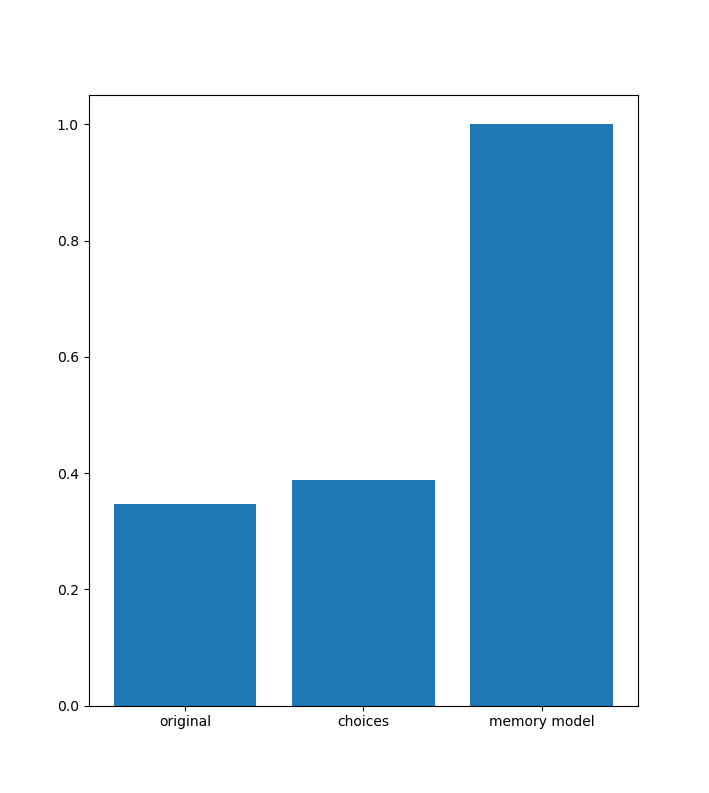
\includegraphics[scale=0.4]{successful_tests.png}
    \caption{The proportion of successful tests out of the 49 synthetic tests created. Tested with the original version of CCF, CCF with the choice-out-of-k nodes, and CCF with choice-out-of-k and the memory model. The memory model clearly results in an increase in the ability to detect memory bugs.}
    \label{fig:successful-tests}
\end{figure}

Figure \ref{fig:successful-tests} shows the results of executing the synthetic test suite with the original version of CCF, modified to include some bug fixes, CCF with choice-out-of-k nodes implemented but using a behaviour-less dummy memory model, and CCF with choice-out-of-k nodes and the array memory model implementation. We can see that the original version of CCF passes 17 out of 49 tests, corresponding to the tests that ensure no error is reported for correct program behaviour. This is the expected result as CCF does not use a memory model implementation so it should not produce any errors. With the implementation of the array memory model, the ability to detect memory bugs is greatly increased and CCF is able to correctly produce error messages for all tests that contain errors. This shows that the implementation of the array memory model matches the design of the array memory model described earlier.

\begin{figure}
    \centering
    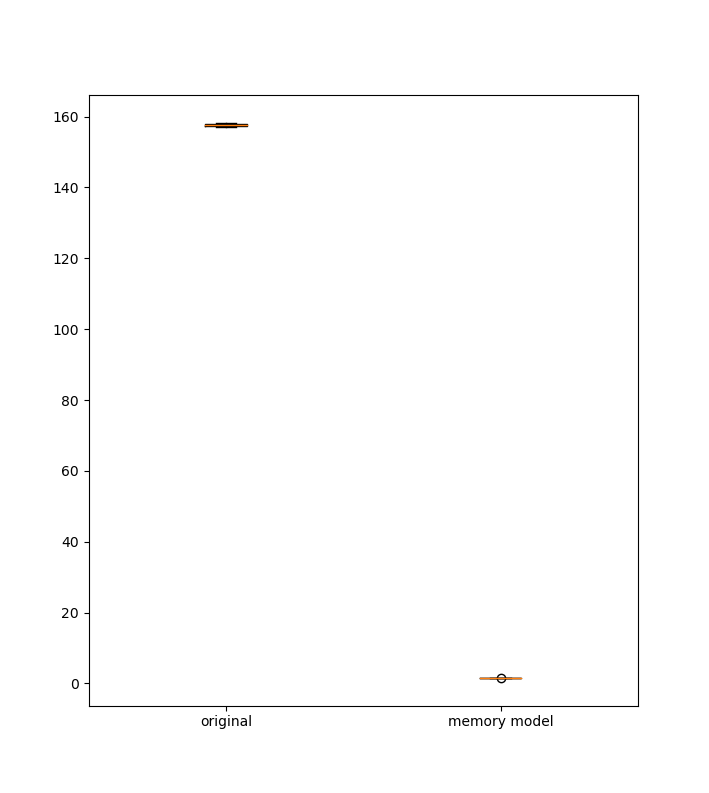
\includegraphics[scale=0.4]{switch-compile-times.png}
    \caption{The time taken to compile a program containing a large switch statement using the original version of CCF and CCF with the array memory model and choice-out-of-k nodes. Each box-plot shows the compile times from a sample of 30 compilations.}
    \label{fig:switch-compile-times-figure}
\end{figure}

Figure \ref{fig:switch-compile-times-figure} shows how the implementation of choice-out-of-k nodes makes compiling large switch statements significantly faster. We would expect this as the previous algorithm to convert switches into binary choices emitted $\mathcal{O}(n^2)$ binary constraints in total while using choices only requires us to emit $\mathcal{O}(n)$ constraints. As well as giving a large speed-up this also means that programs that use significantly larger switches can now be compiled, as in testing we found that clang would fail to instrument very large switch statements with the original version of CCF. 


\begin{figure}
    \centering
    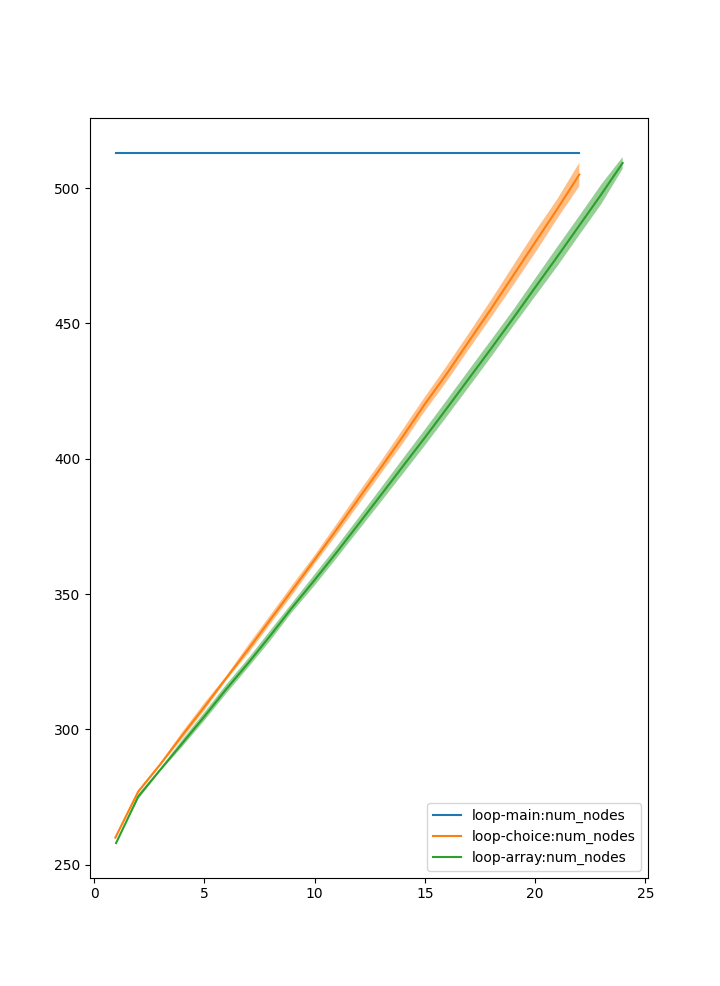
\includegraphics[scale=0.4]{loop-num-nodes.png}
    \caption{The mean number of nodes generated over the runtime of a simple loop with a confidence interval of 99.7\%. Each test was run 30 times.}
    \label{fig:loop-num-nodes}
\end{figure}

\begin{figure}
    \centering
    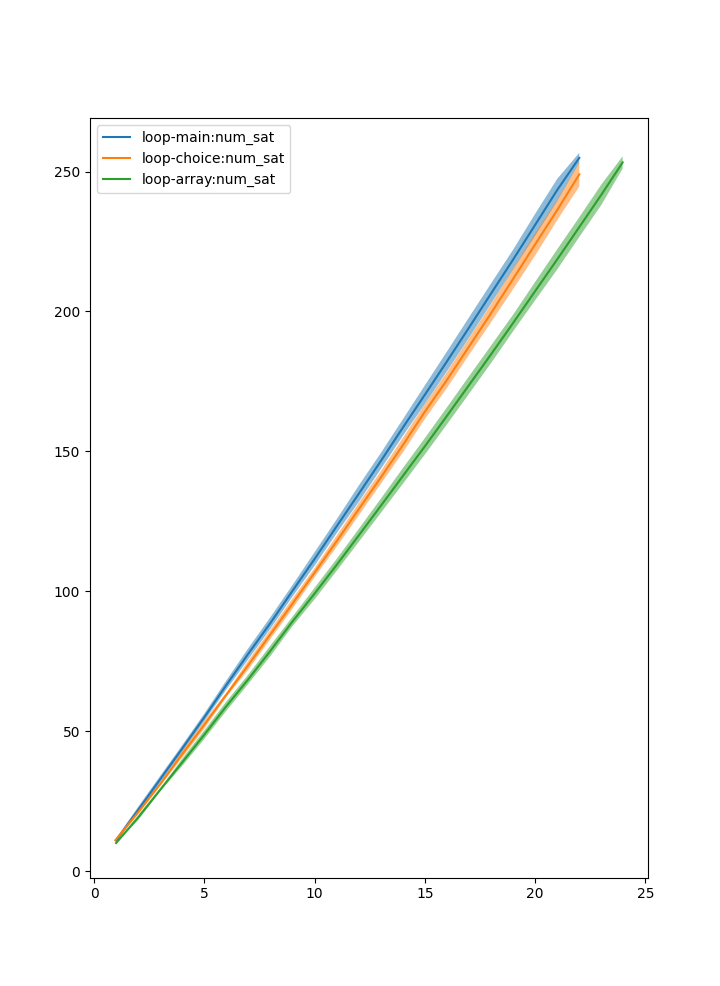
\includegraphics[scale=0.4]{loop-num-sat.png}
    \caption{The mean number of satisfied nodes generated over the runtime of a simple loop with a confidence interval of 99.7\%. Each test was run 30 times.}
    \label{fig:loop-num-sat}
\end{figure}

Figures \ref{fig:loop-num-nodes, fig:loop-num-sat} show the performance of running CCF on a simple program that loops until the loop counter equals a symbolic variable.
We can see that adding the array memory model introduces a statistically significant overhead but the overall performance is comparable.

Figure \ref{fig:loop-num-nodes} shows the number of nodes in the execution tree over time. We see that the original version of CCF creates all the nodes immediately, while the versions with choice-out-of-k add the nodes gradually over time. This doesn't have a significant impact on the performance of the program, but for larger programs could save resources by only adding nodes when needed. Importantly, the choice-out-of-k versions never add unsatisfiable nodes which could waste a significant amount of memory in the original version.

Figure \ref{fig:loop-num-sat} shows the number of nodes explored over time. We see that the original version and the version with choices but without the array memory model have similar performance, while adding the array memory model is slower. This is expected as adding the array memory model requires the program to do more work in creating extra constraints and solving more complex SMT queries. The test program only uses binary branches, so it is good to see that the performance has not significantly degraded when using choice-out-of-k nodes for the binary case. As the binary case is the most common type of branch, it is important that we maintain good performance for this case and the fact that it is possible to generalise branches to allow any number of nodes without making this case perform worse justifies the implementation of choices.


\section{Threats to Validity}
One concern may be that the implementation of the array memory model may not match the design of the memory model. As the synthetic test suite tests the behaviour of each core function of the array memory model implementation and we pass all the synthetic tests we are confident that the implementation matches the design.



%%%%%%%%%%%%%%%%%%%%%%%%%%%%%%%%%%%%
\chapter{Conclusion}
We have discussed several ways to implement a memory model for concolic execution. From this we have identified an array model as an achievable goal to implement for the CCF concolic executor. This will enable us to detect memory bugs in C programs by tracking memory accesses and should allow us to discover new, interesting inputs for the program though the concolic paradigm. A successful project will be able to detect a range of memory bugs implanted into a suite of test programs, demonstrating that we are able to distinguish which bugs are present in a given C program.

\section{Future Work}
Implement the theory of arrays
Implement provenance


%% bibliography
\bibliography{references}


\end{document}
